\chapter{非ユークリッド解析幾何学}

通常の極座標 $\rho$ と $\theta$ を用いる。点の直交座標 $x$ と $y$ としては、その点から軸に下ろした垂線が軸上に切り取る切片を用いる。公式は三角法の関係に依存し、二つの幾何学では、線の長さに虚数因子 $i$ をつけるかどうかだけが異なる。

\section{双曲解析幾何学}

\begin{figure}[h]
\centering
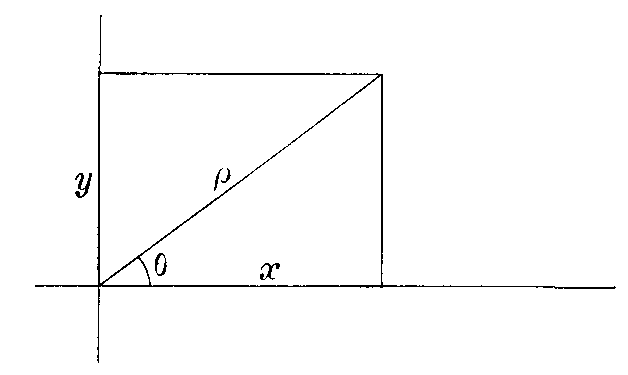
\includegraphics[width=60mm]{fig61.png}
\end{figure}

\begin{description}
\item[1.~極座標と直交座標の関係:]\hfill\break

原点で動径が軸となす角は余角である。二つの直角三角形から、
\begin{align*}
\tan ix &= \cos\theta \tan i\rho, \\
\tan iy &= \sin\theta \tan i\rho. \\
\intertext{したがって、}
\tan^2 i\rho &= \tan^2 ix + \tan^2 iy, \\
\tan\theta &= \frac{\tan iy}{\tan ix}.
\end{align*}

\begin{figure}[h]
\centering
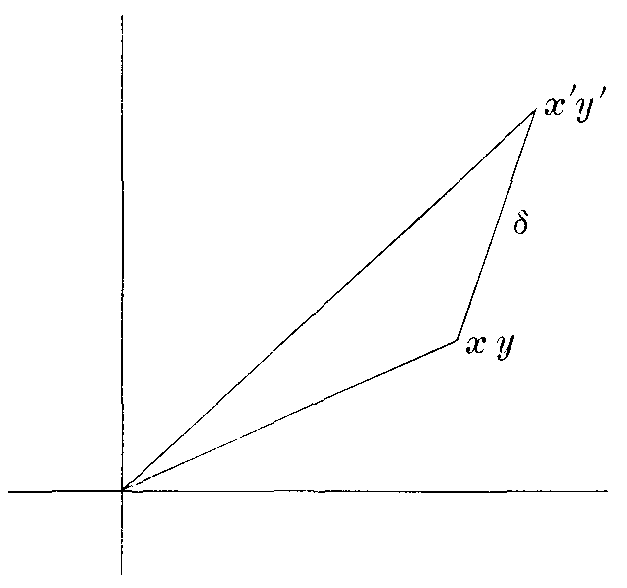
\includegraphics[width=60mm]{fig62.png}
\end{figure}

\item[2.~二点間の距離 \boldmath$\delta$:]

\begin{equation*}
\cos i\delta = \cos i\rho\, \cos i\rho'
                + \sin i\rho\, \sin i\rho'\, \cos(\theta'-\theta).
\end{equation*}
$\delta$ と一方の点を固定すれば、これは円の極方程式とみなせる。

\begin{figure}[h]
\centering
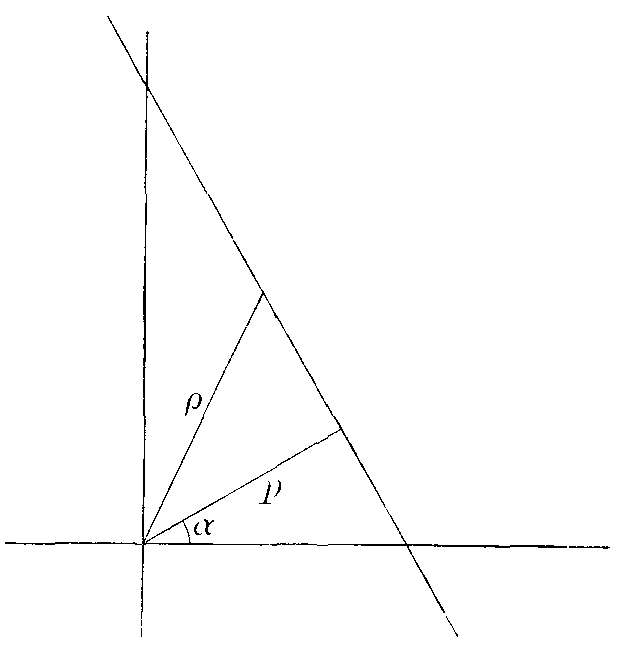
\includegraphics[width=60mm]{fig63.png}
\end{figure}

\item[3.~直線の方程式:]\hfill\break

\textbf{$p$} を原点から直線に下ろした垂線の長さ、$\alpha$ をこの垂線が $x$ 軸となす角とする。この垂線と $\rho$ でできる直角三角形から、
\begin{equation*}
\tan i\rho\, \cos(\theta-\alpha) = \tan ip
\end{equation*}
を得る。これは直線の極方程式である。展開して代入することにより、$x$ と $y$ の方程式
\begin{equation*}
\cos\alpha\,\tan ix + \sin\alpha\,\tan iy = \tan ip
\end{equation*}
を得る。

方程式 $a\tan ix + b\tan iy = i$ は、
\begin{equation*}
a^2 + b^2 = \frac{-1}{\tan^2 ip}
\end{equation*}
である直線を表す。ところで、$p$ の実数値に対して $-\tan^2ip < 1$ である（前出の脚注を見よ）。したがって直線が実であるのは、$a$ と $b$ が実数で、
\begin{equation*}
a^2 + b^2 > 1
\end{equation*}
であるときである。

\begin{figure}[h]
\centering
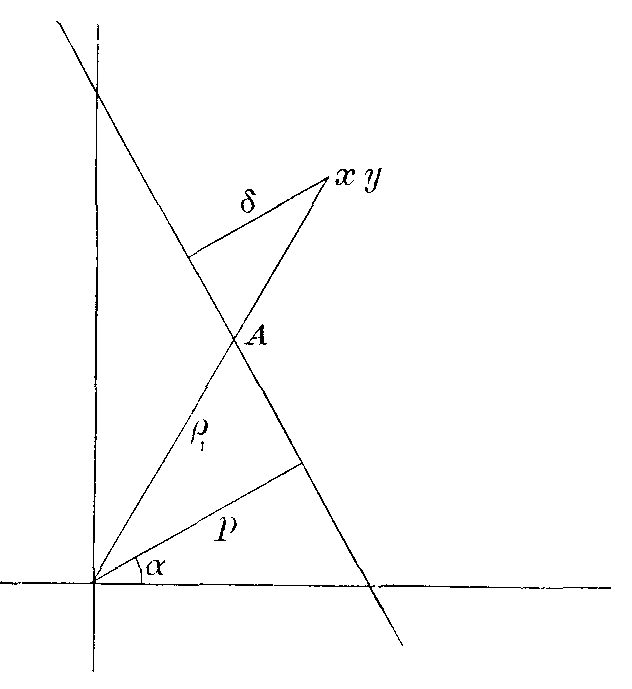
\includegraphics[width=60mm]{fig64.png}
\end{figure}

\item[4.~点から直線までの距離 \boldmath$\delta$:]\hfill\break

その点への動径が直線と $A$ で交わるとし、$\rho_1$ を $A$ への動径とする。$A$ で等しい角をもつ二つの直角三角形があり、これらの角の正弦の表式から方程式
\begin{equation*}
\frac{\sin i\delta}{\sin i(\rho-\rho_1)} =
                                        \frac{\sin ip}{\sin i\rho_1}
\end{equation*}
を得る。この方程式は平面のすべての点 $x\,y$ について成り立つ。$\delta$ は、点が原点と直線の同じ側にあるときは負であり、点が直線上にあるときは零である。
\begin{equation*}
\sin i\delta
   =\frac{\sin ip}{\tan i\rho_1}\sin i\rho-\sin ip\,\cos i\rho.
\end{equation*}

さて、
\begin{align*}
\tan i\rho_1 &= \frac{\tan ip}{\cos(\theta-\alpha)}. \\
\therefore \frac{\sin ip}{\tan i\rho_1}\sin i\rho
           &=\sin i\rho\,\cos ip\,\cos(\theta-\alpha), \\
\intertext{および}
 \sin i\delta &= \cos i\rho\, \cos ip\,
   \left[\tan i\rho\, \cos(\theta-\alpha) - \tan ip\right].
\end{align*}
$\delta$ を固定すれば、これは等距離曲線の極方程式とみなせる。

\begin{figure}[ht]
\centering
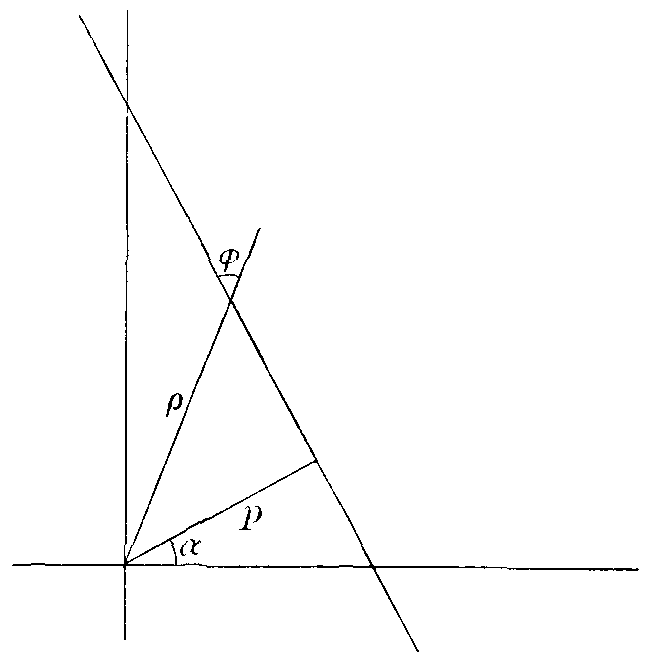
\includegraphics[width=60mm]{fig65.png}
\end{figure}

\item[5.~二直線のなす角:]\hfill\break

$\phi$ を、直線が任意の点で動径となす角とすると、
\begin{align*}
 \cos \phi &= \cos ip\, \sin (\theta-\alpha),\\
 \sin \phi &= \frac{\sin ip}{\sin i\rho}.
\end{align*}

この点で交わる二直線については、
\begin{align*}
 \sin \phi_1\, \sin \phi_2 &= \frac{\sin ip_1\, \sin ip_2}{\sin^2 i\rho}\\
 &= \sin ip_1\, \sin ip_2 + \frac{\sin ip_1\, \sin ip_2}{\tan^2 i\rho}.
\end{align*}

さて、直線の方程式から、
\begin{align*}
\frac{\sin ip_1}{\tan i\rho} &= \cos ip_1\, \cos(\theta-\alpha_1),\\
\frac{\sin ip_2}{\tan i\rho} &= \cos ip_2\, \cos(\theta-\alpha_2);\\
\intertext{したがって}
\sin \phi_1 \sin \phi_2 &= \sin ip_1\, \sin ip_2
   + \cos ip_1\, \cos ip_2\, \cos(\theta-\alpha_1)\,\cos(\theta-\alpha_2).\\
\intertext{またさらに、}
\cos \phi_1\, \cos \phi_2 &= \cos ip_1\, \cos ip_2\, \sin
  (\theta-\alpha_1)\,\sin (\theta-\alpha_2). \\
\intertext{これらの式を加えると、}
\cos (\phi_2-\phi_1) &= \sin ip_1\, \sin ip_2 +
        \cos ip_1\, \cos ip_2\, \cos (\alpha_2-\alpha_1).
\end{align*}

二直線が垂直であるのは、
\begin{align*}
\cos (\alpha_2-\alpha_1) + \tan ip_1\, \tan ip_2 &= 0 \\
\intertext{のときである。直線}
 a \tan ix + b \tan iy &= i,\\
 a' \tan ix + b' \tan iy &= i, \\
\intertext{が垂直であるのは、}
aa' + bb' &=1
\end{align*}
のときである。

\item[6.~円の $x$ と $y$ による方程式:]

\begin{align*}
 \sin i\rho\, \cos \theta &= \cos i\rho\, \tan ix,\\
 \sin i\rho\, \cos \theta &= \cos i\rho\, \tan iy;
\intertext{また、}
 \cos i\rho &= \frac{1}{\sqrt{1+\tan^2 i\rho}} =
\frac{1}{\sqrt{1+\tan^2 ix+\tan^2 iy}}.
\end{align*}

したがって、円の方程式は次のように書ける。
\begin{multline*}
  (1 + \tan^2ix + \tan^2iy)
  (1 + \tan^2ix' + \tan^2iy') \cos^2i\delta\\
  = (1 + \tan ix \tan ix' + \tan iy \tan iy')^2.
\end{multline*}

\begin{figure}[h]
\centering
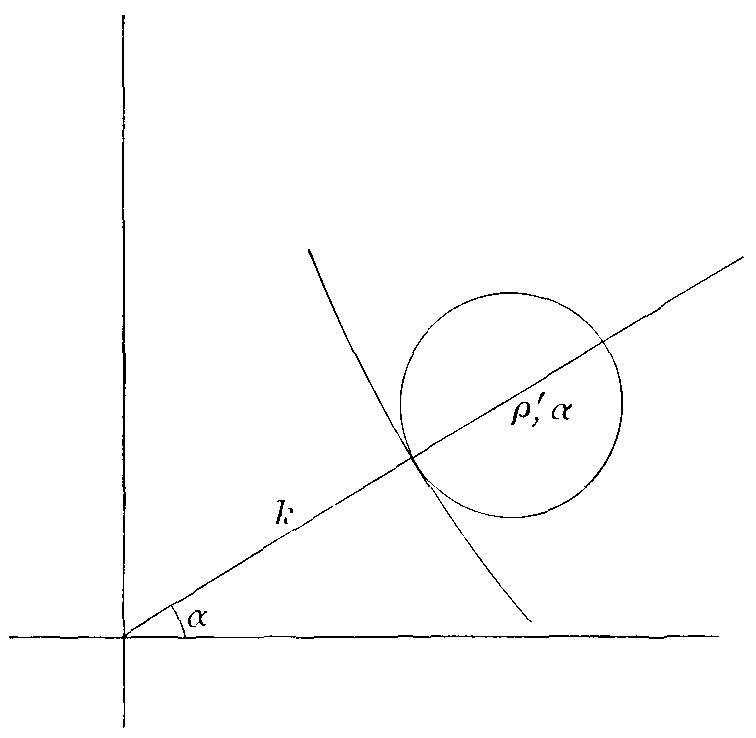
\includegraphics[width=60mm]{fig66.png}
\end{figure}

\item[7.~限界曲線の方程式:]\hfill\break

\textbf{原点}を通る限界曲線の軸が $x$ 軸と角 $\alpha$ をなすとし、限界曲線がこの軸と交わる点が原点から距離 $k$ にあるとする。$k$ は、原点が曲線の凸の側にあるときは正、曲線の凹の側にあるときは負とする。限界曲線は、この軸上の中心が限りなく遠ざかるときの円の極限の位置である。

$\rho'$ を中心への動径とすると、円の半径は $\rho'-k$ であり、その方程式は
\begin{equation*}
  \cos i(\rho'-k) = \cos i\rho\, \cos i\rho'
  + \sin i\rho\, \sin i\rho'\, \cos(\theta-\alpha)
\end{equation*}
と書ける。あるいは、展開して $\cos i\rho'$ で割ると、
\begin{equation*}
  \cos ik + \tan i\rho'\, \sin ik
  = \cos i\rho + \sin i\rho\, \tan i\rho'\, \cos(\theta-\alpha).
\end{equation*}

ここで $\rho'$ を限りなく増加させる。$\tan i\rho'$ は極限 $i$ に近づくから、この式の左辺の極限は、
\begin{equation*}
  \cos ik + i\sin ik, \text{ すなわち } e^{-k}
\end{equation*}
であり、曲線の極方程式は、
\begin{equation*}
  e^{-k} = \cos i\rho \left[1 + i\tan i\rho\,\cos(\theta-\alpha) \right]
\end{equation*}
となる。あるいは $x\,y$ 座標では、
\begin{equation*}
  (1 + \tan^2ix + \tan^2iy) e^{-2k}
     = (1 + i\cos\alpha\,\tan ix + i\sin\alpha\,\tan iy)^2.
\end{equation*}

\begin{figure}[h]
\centering
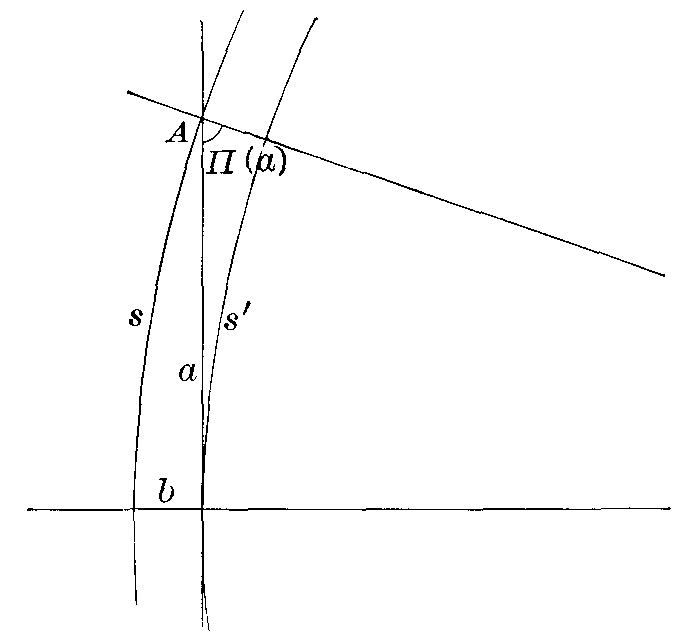
\includegraphics[width=60mm]{fig67.png}
\end{figure}

\textbf{$k$} が負で、たとえば $-b$ に等しいとし、$\alpha=0$ とする。また、$a$ を、曲線が $y$ 軸と交わる点 $A$ の縦座標とする。

方程式に代入すると、
\begin{equation*}
  e^b = \cos ia
\end{equation*}
を得る。

$A$ を通って $x$ 軸に平行に、したがって $y$ 軸と角 $\Pi(a)$ をなす直線を引く。同じ平行線の組を軸とする限界曲線を原点を通って引き、二つの限界曲線がこれらの軸上に距離 $b$ を切り取るようにすれば、対応する弧の比は
\begin{gather*}
  \frac{s'}{s} = \sin\Pi(a) = \frac{1}{\cos ia};
\tag{前出を見よ} \\
\intertext{であることがわかっている。したがって、}
  \frac{s'}{s} = e^{-b}.\tag{前出を見よ}
\end{gather*}

\item[8.~等距離曲線の方程式:]\hfill\break

(4) の極方程式を $x$ と $y$ の方程式に直すと、次の形になる。
\begin{multline*}
  (1 + \tan^2ix + \tan^2iy) \sin^2i\delta \\
  = \cos^2ip (\cos\alpha\,\tan ix + \sin\alpha\, \tan iy -\tan ip)^2.
\end{multline*}

\item[9.~三つの方程式の比較:]\hfill\break

方程式
\begin{equation*}
  (1 + \tan^2ix + \tan^2iy)c^2
     = -(i-a\tan ix -b\tan iy)^2
\end{equation*}
は、それぞれ $a^2+b^2 < 1$、$=1$、$>1$ に応じて、円、限界曲線、等距離曲線を表す。

\begin{figure}[h]
\centering
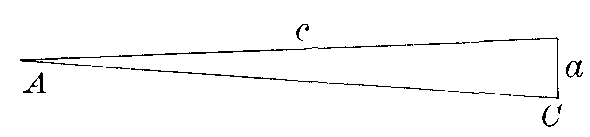
\includegraphics[width=60mm]{fig68.png}
\end{figure}

\item[10.~微分公式:]\hfill\break

頂点の角 $A$ が限りなく小さくなる二等辺三角形を考える。公式
\begin{equation*}
  \frac{\sin A}{\sin ia} = \frac{\sin C}{\sin ic}
\end{equation*}
において、
\begin{center}
\begin{tabular}{ccc}
  $\sin A$, & $\sin ia$, & $\sin C$\\
  の代わりに $A$, & $ia$, & $1$\\
\end{tabular}\\
\end{center}
をそれぞれおくことができる。したがって、
\begin{equation*}
  ia = \sin ic \cdot A.\tag{I.}
\end{equation*}

\textbf{系.} \emph{半径 $\mathbf{r}$ の円において、任意の弧と、中心で張る角との比は $\sin \mathbf{ir}$ である。}

\begin{figure}[h]
\centering
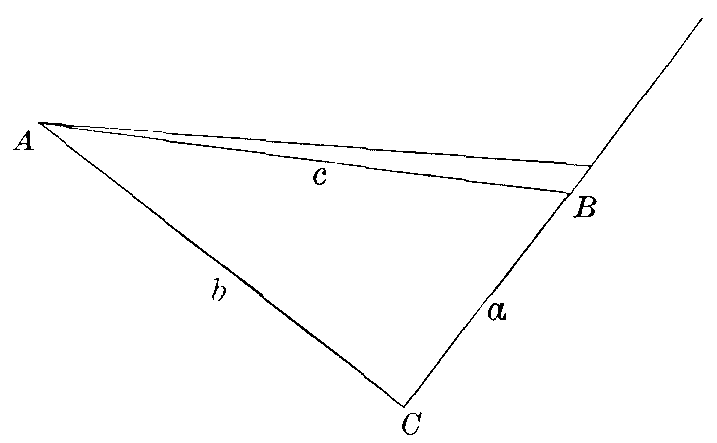
\includegraphics[width=60mm]{fig69.png}
\end{figure}

またさらに、直角三角形 $ABC$ において、斜辺 $c$ を頂点 $A$ のまわりに回転させる。方程式
\begin{align*}
\sin A &= \frac{\cos B}{\cos ib},  \\
\intertext{を（$b$ は定数として）微分すると、}
\cos Ad\,A &= -\,\frac{\sin B\,dB}{\cos ib}.  \\
\intertext{しかるに}
\sin B &= \frac{\cos A}{\cos ia};  \\
\therefore dB &= -\cos ia\, \cos ib\, dA,  \\
\intertext{すなわち（II.）}
dB &= -\cos ic\, dA.
\end{align*}

さて、極座標を用いると、斜辺 $ds$ が動径とたとえば角 $\phi$ をなす無限小の直角三角形ができる（図70を見よ）。直角をはさむ二辺は $d\rho$ と $\frac{\sin i\rho}{i} d\theta$ であるから、
\begin{align*}
ds^2 &= d\rho^2 - \sin^2i\rho\, d\theta^2,  \\
\tan\phi &= \frac{\sin i\rho}{i}\, \frac{d\theta}{d\rho}.
\end{align*}

\begin{figure}[h]
\centering
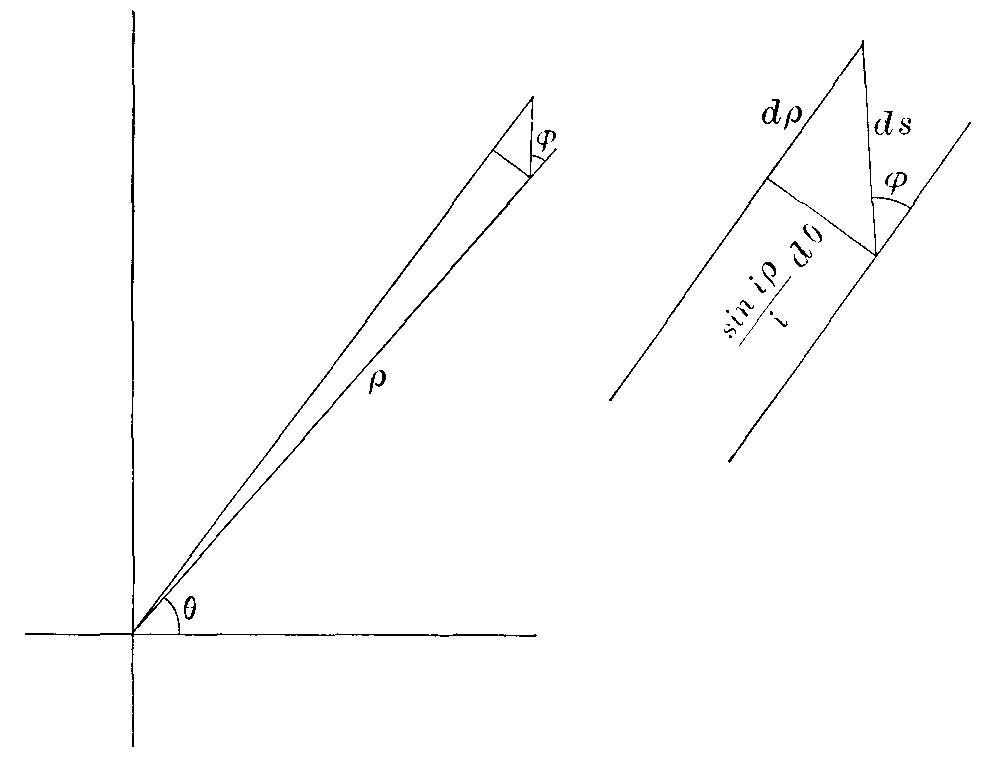
\includegraphics[width=80mm]{fig70.png}
\end{figure}

直角に交わる二つの弧について、$d'$ で第二の弧に沿った微分を表す。
\begin{align*}
  \frac{\sin i\rho}{i}\, \frac{d\theta}{d\rho}
  &= -\, \frac{i}{\sin i\rho}\, \frac{d'\rho}{d'\theta},\\
\intertext{すなわち}
  \frac{d\rho}{d\theta}\, \frac{d'\rho}{d'\theta}
  &= \sin^2i\rho.
\end{align*}

\item[11.~面積:]\hfill\break

面積は
\begin{equation*}
  \iint \frac{\sin i\rho}{i}\, d\rho\, d\theta
\end{equation*}
に等しい。\footnote{面積の単位は、無限小の長方形の面積が、その底辺と高さの積で表されるように選ぶ。}

原点が計算する面積の内部にあって、各動径が境界の曲線とただ一度だけ交わる場合のみを考える。

$\rho$ について $\rho=0$ から積分すると、
\begin{align*}
  \int_0^{2\pi} (\cos i\rho - 1) d\theta,\\
  \intertext{すなわち}
  \int_0^{2\pi} \cos i\rho\, d\theta - 2\pi
\end{align*}
を得る。

\begin{figure}[h]
\centering
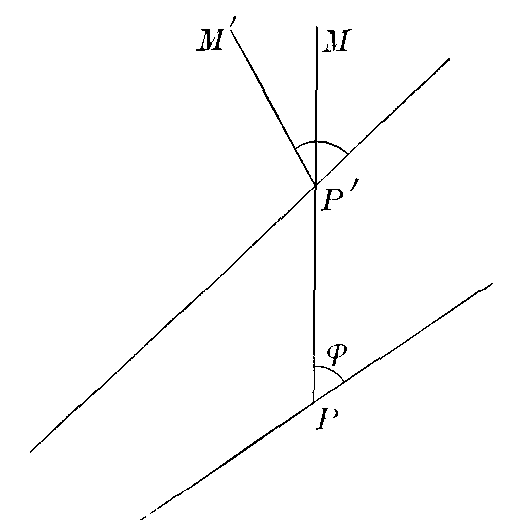
\includegraphics[width=60mm]{fig71.png}
\end{figure}

$P$ と $P'$ を曲線上の二つの「隣り合う」点とし、$PM$ と $P'M'$ をそれらの点での接線とし、$\phi$ を接線が動径となす角とする。角 $MP'M'$ は、曲線を一周するときのこれらの点での回転の量を表す。

さて、(II.) により、
\begin{equation*}
  MP'M' = d\phi + \cos i\rho\, d\theta.
\end{equation*}

曲線を一周するとき、$\phi$ は変化しうるが、最後にはもとの値に戻る。すなわち、この曲線については、
\begin{gather*}
  \int d\phi = 0, \\
\intertext{であり、回転の量は}
  \int_0^{2\pi} \cos i\rho\, d\theta
\end{gather*}
である。

ゆえに、面積は、曲線を一周するときの回転の量の、四直角を超える過剰に等しい。この定理は、任意の有限な面積に拡張できる。

\item[12.~座標系の修正:]\hfill\break

$\tan ix$ の代わりに $iu$、$\tan iy$ の代わりに $iv$、$\tan i\rho$ の代わりに $ir$ と書き、以下すべての線の長さについても同様にすると、方程式は簡単な形になる。

すると、
\begin{align*}
u^2 + v^2 &= r^2.\footnotemark \\
\intertext{直線の方程式は}
au + bv &= 1, \\
\intertext{であり、方程式}
(1 - u^2 - v^2)c^2 &= (1 - au - bv)^2
\end{align*}
は、それぞれ $a^2+b^2<1$、$=1$、$>1$ に応じて、円、限界曲線、等距離曲線を表す。
\footnotetext{三つの直角をもつ四角形を描き、鋭角への対角線を引いて、$a$、$b$、$c$ を上の $u$、$v$、$r$ と同じように用いれば、図に記した五つの部分は、ユークリッド幾何学の直角三角形の関係をもつ。たとえば、
\begin{equation*}
a^2 + b^2 = c^2 , \sin A = \frac{a}{c}, \text{など}.
\end{equation*}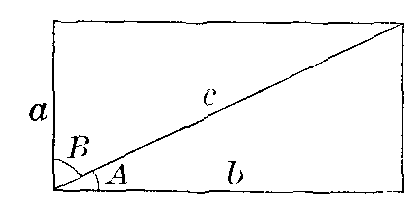
\includegraphics[width=25mm]{fig73.png}}
\end{description}

